\chapter{Paramètres et Valeur de retour}
\label{chap:Parametres}

Afin de permettre à notre code d'intéragir avec le moteur de jeu, il faut utiliser une fonction :

\begin{listing}[!htpb]
    \begin{minted}{c}
        action lode_runner(levelinfo, character_list, bonus_list, bomb_list);
    \end{minted}
    \caption{Prototype de \texttt{lode\_runner} en C.}
    \label{listing:c-lode_runner-prototype}
\end{listing}

\section{Paramètres}

\begin{table}[!htpb]
    \label{tab:parameters-lode_runner}
    \begin{tabularx}{\textwidth}{lXr}
        \toprule
        \textbf{Paramètre} & \textbf{Type} & \textbf{Description} \\
        \midrule
        \texttt{level} & \texttt{levelinfo} & Structure contenant les informations du niveau. \\
        \texttt{characterl} & \texttt{character\_list} & Liste chaînée contenant le runner et les ennemis. \\
        \texttt{bonusl} & \texttt{bonus\_list} & Liste chaînée contenant les bonus. \\
        \texttt{bombl} & \texttt{bomb\_list} & Liste chaînée contenant les bombes. \\
        \bottomrule
    \end{tabularx}
    \caption{Paramètres de la fonction \texttt{lode\_runner}.}
\end{table}

\section{Valeur de retour}

Cette fonction est appellée à chaque tour du jeu. Elle retourne une action à effectuer par le runner.
Cette action est un élément de l'énumération suivante :

\begin{table}[!htpb]
    \label{tab:enum-action}
    \begin{tabularx}{\textwidth}{lXX}
        \toprule
        \textbf{Entier} & \textbf{Valeur} & \textbf{Description} \\
        \midrule
        0 & \texttt{NONE} & Ne rien faire. \\
        1 & \texttt{UP} & Aller en haut. \\
        2 & \texttt{DOWN} & Aller en bas. \\
        3 & \texttt{LEFT} & Aller à gauche. \\
        4 & \texttt{RIGHT} & Aller à droite. \\
        5 & \texttt{BOMB\_LEFT} & Poser une bombe à gauche. \\
        6 & \texttt{BOMB\_RIGHT} & Poser une bombe à droite. \\
        \bottomrule
    \end{tabularx}
    \caption{Énumération des actions possibles.}
\end{table}

\newpage

\section{Struture \texttt{levelinfo}}

Parmi les paramètres de la fonction \texttt{lode\_runner}, il y a la structure \texttt{levelinfo}.
Cette structure contient les informations du niveau actuel, sous la forme suivante :

\begin{listing}[!htpb]
    \begin{minted}{c}
        typedef struct{
            char **map;
            int xsize;
            int ysize;
            int xexit;
            int yexit;
        } levelinfo;
    \end{minted}
    \caption{Structure \texttt{levelinfo} en C.}
    \label{listing:c-levelinfo-struct}
\end{listing}

Le tableau \texttt{map} contient les éléments de la carte, sous la forme d'un tableau de caractères, un exemple est donné sur la \autoref{fig:map1}.

\begin{figure}[!htpb]
    \centering
    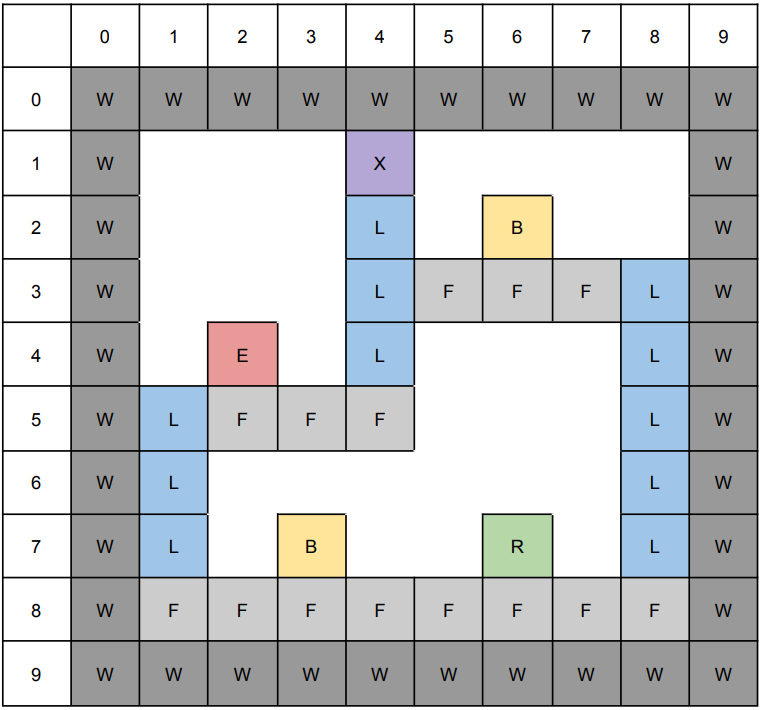
\includegraphics[width=\linewidth]{Figures/map1.png}
    \caption[Exemple de carte.]{Exemple de carte.}
    \label{fig:map1}
\end{figure}

\newpage

On peut remarquer que les \texttt{x} et les \texttt{y} sont inversés par rapport à une matrice classique, c'est à dire que l'axe des ordonnées est l'axe des abscisses et vice-versa.
De plus, les coordonnées sont relatives à la carte, c'est à dire que le coin supérieur gauche est en (0, 0) et le coin inférieur droit est en (\texttt{xsize}, \texttt{ysize}).
Enfin, cela mène à ce que contrintuitivement, se déplacer vers le haut signifie diminuer les \texttt{y}.

Afin de faciliter le développement, et de laisser une liberté de choix dans l'implémentation, chaque caractère de la carte est défini par une constante, comme suit :

\begin{table}[!htpb]
    \label{tab:enum-tile}
    \begin{tabularx}{\textwidth}{lXX}
        \toprule
        \textbf{Caractère} & \textbf{Constante} & \textbf{Description} \\
        \midrule
        'H' & \texttt{BOMB} & Bombe. \\
        'B' & \texttt{BONUS} & Bonus. \\
        'C' & \texttt{CABLE} & Câble. \\
        'E' & \texttt{ENEMY} & Ennemi. \\
        'X' & \texttt{EXIT} & Sortie. \\
        'F' & \texttt{FLOOR} & Sol. \\
        'L' & \texttt{LADDER} & Échelle. \\
        '.' & \texttt{PATH} & Chemin. \\
        'R' & \texttt{RUNNER} & Runner. \\
        'W' & \texttt{WALL} & Mur. \\
        \bottomrule
    \end{tabularx}
    \caption{Énumération des caractères de la carte.}
\end{table}